\documentclass{article}
\usepackage[margin=1in]{geometry}
\usepackage{../common}
\usepackage{../pagesetup}
\usepackage{xcolor}

% **** IF YOU WANT TO DEFINE ADDITIONAL MACROS FOR YOURSELF, PUT THEM HERE:
\renewcommand{\v}{\boldsymbol}
\newcommand{\argmax}{arg\,max}
\begin{document}

\lecture{5}{September 18}{Sasha Rush}{Demi Guo, Artidoro Pagnoni, Luke Melas-Kyriazi }{Linear Classification}

\subsection{Classification Introduction}
Last time we saw linear regression. In linear regression we were predicting $y \in \mathbb{R}$, in classification instead we deal with a discrete set, for example $y \in \{ 0,1\}$ or $y\in \{1, \ldots, C\}$. This distinction only matters for this lecture, starting from next class we will generalize the topics and treat them as the same thing.

\smallskip

Among the many applications, linear classification is used in sentiment analysis, spam detection, and facial and image recognition. We will use generative models of the data, which means that we will model both the $x$ and the $y$ explicitly, and we are not keeping $x$ fixed. In the case of the spam filter earlier, $x$ is the email body, and $y$ is the label $\{$spam, not spam$\}$. A generative model of the email and labels, we would model the distribution of $x$, of the text in the email itself, and not only the distribution of the category $y$.

\smallskip

We will explore the basic method of Na\"ive Bayes in detail. Even with a very simple method like Na\"ive Bayes with basic features it is possible to perform extremely well on many classification tasks when large training data sets are available. For example, this simple model performs almost as well (one percent point difference) as very complex methods on spam detection.

\subsection{Na\"ive Bayes}
Note that the term "Bayes" in Na\"ive Bayes (NB) does not have to do with Bayesian modeling, or the presence of priors on parameters. We won't have any priors for the moment.  General Na\"ive Bayes takes the following form:
\begin{align*}
    y &\sim \on{Cat}(\pi) ~~~~~~~~~~~~~ \text{[class distribution]}\\
    \v x|y &\sim \prod_{j}p(x_j \mid y) ~~~~~ \text{[class conditional]}
\end{align*}
where $y$ is the class label and comes from a categorical distribution, and $x_j$ is a dimension of the input $x$.

\smallskip

In Na\"ive Bayes, the form of the class distribution is fixed and parametrized independently from the class conditional distribution. The "Na\"ive" term in "Na\"ive Bayes" precisely refers to the conditional independence between $y$ and $x_j|y$. Depending of what the data looks like we can choose a different form for the class conditional distribution.

\smallskip

Here we present three possible choices for the class conditional distribution:

\begin{itemize}
    \item \textbf{Multivariate Bernoulli Na\"ive Bayes}:  
    $$ x_j|y \sim \on{Bern}(\mu_{jc}) ~~~~~~\text{if $y=c$} $$
    Here $y$ takes values in a set of classes, and $\mu_{jc}$ is a parameter associated with a specific feature (or dimension) in the input and a specific class. We use multivariate Bernoulli when we only allow two possible values for each feature, therefore $x_j|y$ follows a Bernoulli distribution.
    
    We can think of $x$ as living in a hyper cube, with each dimension $j$ having an associated $\mu$ for each class $c$. From here we get the name multivariate Bernoulli distribution. 

    \item \textbf{Categorical Na\"ive Bayes}:
    $$ x_j|y \sim \on{Cat}(\mu_{jc}) ~~~\text{if $y=c$} $$
    We use the Categorical Na\"ive Bayes when we allow different classes for each feature $j$, so $x_j|y$ follows a Categorical distribution.

    \item \textbf{Multivariate Normal Na\"ive Bayes}
    $$ \v x|y \sim \mathcal{N}(\v \mu_c, \mathbf{\Sigma}_{diag}^c) $$
    Note that here we use $\v x$ vector and not a specific feature. Since we impose that $\v \Sigma^c$ is a diagonal matrix, we have no covariance between features, so this comes down to having an independent normal for each feature (or dimension) of the output. This is also required by the "Na\"ive" assumption of conditional independence. We would use  MVN Na\"ive Bayes when the features take continuous values in $\mathbb{R}^n$. 
\end{itemize}    
        
\subsection{General Na\"ive Bayes}
We consider the data points $\{(\v x_n,y_n)\}$, without specifying a particular generative model. The likelihood of each data point is:
\begin{align}
    p(\v x_n,y_n | \text{param}) &= p(y_n|\v \pi)\prod_j p(x_{nj}|y_n, \text{param})\\
    &= \prod_c \pi_c^{(y_n = c)} \prod_j \prod_c p(x_{nj}|y_n)^{(y_n=c)}
\end{align}
where in equation (5.2) we assume conditional independence (the "Na\"ive" assumption). The term $p(x_{nj}|y_n)$ depends on the generative model used for $x$ and also on the class $y_n$.

\smallskip

We can then solve for the parameters maximizing the likelihood, which is equivalent to maximizing the $\log$ likelihood.
\begin{align}
		\left(\pi_{\on{MLE}}, \mu_{\on{MLE}}\right) &= \underset{(\v \pi,\v \mu)}{\on{argmax}} \sum_n \log p(\v x_n , y_n| \text{param})\\
		&= \underset{(\v \pi,\v \mu)}{\on{argmax}} \sum_c N_c \log \pi_c + \sum_i\sum_c\sum_{n:y_n=c}\log p(x_{nj}|y_n)\\
	    &= \left(\arg\!\max_{(\v \pi,\v \mu)} \sum_c N_c \log \pi_c\right) + \left(\arg\!\max_{(\v \pi,\v \mu)} \sum_i\sum_c\sum_{n:y_n=c}\log p(x_{nj}|y_n)\right)
\end{align}
Where $N_c = \sum_n \mathbb{1}(y_n = c)$, and $N =$ the number of data points.

\smallskip

This factors into two parts (5.10), the first only depending on $\v\pi$ the other is the MLE for the class condition distribution on each feature or dimension of the input. This factorization allows to solve for the maximizing $\v\pi$ and the maximizing parameters for the class conditional separately.

\smallskip

For example, if we use a Multivariate Bernoulli Na\"ive Bayes generative model we would get the following parameters from MLE:
\begin{align}
		\pi_c &= \frac{N_c}{N}\\
		\mu_{jc} &= \frac{\sum_{n:y_n=c}x_{nj}}{N_c} = \frac{N_{cj}}{N_c}
\end{align}
Again, where $N_c = \sum_n \mathbb{1}(y_n = c)$, $N_{cj} = \sum_n \mathbb{1}(y_n = c) x_{nj}$ and $N =$ number of data points.\\
\subsection{Bayesian Naive Bayes: Add a Prior}
Here, instead of working with a single distribution, we are working with multiple distributions. For simplicity, let's use the following factored \textbf{prior}:
\[p(\pi, \mu) = p(\pi) \prod_j \prod_c p(\mu_{jc})\] 
where $p(\pi)$ represents the prior on class distribution and $\prod_j \prod_c p(\mu_{jc})$ represents prior on class conditional distribution.

\smallskip

Now, \textbf{what prior should we use?}
\begin{enumerate}
    \item $\pi$: Dirichlet (goes with Categorical)
    \item $\mu_{jc}$: 
        \begin{enumerate}
            \item Beta (goes with Bernoulli)
            \item Dirichlet (goes with Categorical)
            \item Normal (goes with Normal)
        \end{enumerate}
        Here, what distribution we choose depends on our choice of class conditional distribution.
\end{enumerate} 
Recall that we want to use conjugate priors to have a natural update (that's why we pair them up!). By using conjugate priors, we will have:
    \[ p(\pi | \text{data}) = Dir(N_1 + \alpha_1, \cdots, N_c + \alpha_c) \]
    \[ p(\mu_{jc} | \text{data}) = \beta((N_c - N_{jc}) + \beta_0, N_c + \beta_1) \]
\subsubsection{Intuition}
You can think of the $\alpha_i$ above as initial pseudocounts. Those pseudocounts give nonzero probability to features we haven't seen before, which is crucial for NLP. For unseen features, you could have a pseudocount of 1 or 0.5 (Laplace term) or something. 

Because of this property, a Bayesian model helps prevents overfitting by introducing such priors: consider the spam email classification problem mentioned before. Say the word "subject" (call it feature $j$) always occurs in both classes ("spam" and "not spam"), so we estimate $\hat{\theta}_{jc} = 1$ (we overfit!) What will happen if we encounter a new email which does not have this word in it? Our algorithm will crash and burn! This is another manifestation of the black swan paradox discussed in Book Section 3.3.4.1. Note that this will not happen if we introduce pseudocounts to all features! 
\subsection{Posterior Predictive}
\[p(\hat{y}, \hat{x} \mid \text{data}) = (\text{integrate over parameters})\] 
\[ {\pi_c}^{\on{MAP}} = \frac{N_c + \alpha_c}{N + \sum_c \alpha_c} (\text{Dirichlet MAP}) \] 
\[{\mu_{jc}}^{\on{MAP}} = \frac{N_{jc} + \beta_1}{N_c + \beta_1 + \beta_0} (\text{Beta MAP})\] 
(How to derive this? Good exercise!)
\subsection{More on Predictive}
Now, let's consider a little bit more about what's happening in our predictive. Consider the email spam classification problem: given some features of an email, we want to predict if the email is a spam or not a spam. We have:
\begin{align*}
    p(y = c | x, data) &\propto \pi_c \prod_j p(x_j|y) \> (\text{try to generate observations from class}) \\
    &= \pi_c \prod_j \mu_{jc}^{x_j} (1-\mu_{jc})^{(1-x_j)} \> (\text{informal parametrization})\\
    &= \exp(\log \pi_c + \sum_j x_j \log \mu_{jc} + (1-x_j) \log(1 - \mu_{jc})) \> (\text{take exp of log})\\
    &= \exp\left(\log \pi_c + \sum_j \log(1-\mu_{jc}) + \sum_j x_j \log\frac{\mu_{jc}}{1-\mu_{jc}}\right)
\end{align*}
where the first two term $log \pi_c + \sum_j log(1-\mu_{jc})$ is a constant (we call it $b$ for bias), and the last term $\sum_j x_j log\frac{\mu_{jc}}{1-\mu_{jc}}$ is linear (we call it $\theta$).
\subsection{Multivariate Bernoulli Naive Bayes}
For Multivariate Bernoulli NB, we will have:
\begin{align*}
    \theta_{jc} &= \log \frac{\mu_{jc}}{1 - \mu_{jc}} \\
    b_c &= \log \pi_c + \log(1- \mu_{jc})
\end{align*}
So, we have:
$$ p(y=c \mid x) \propto \exp(\theta_c^T x + b_c) $$
Thus, in order to determine which class ("spam" or "not spam"), for each class we simply compute a linear function with respect to x, and compare the two. Our $\theta x + b$ is going to be associated with a linear separator of the data.  Even better, for prediction, we can simply compute $\theta$ and $\beta$ (as shown above) using closed form for both MAP and MLE cases.

\subsection{The Sigmoid Function}
Before proceeding, we should name our variables to speak about them more easily.

\smallskip

We call $\mu$ the "informal parameters" and $\theta$ the "scores." In the case of a Multivariate Bernouli model, we have the map $\theta_{jc} =  \log \frac{\mu_{jc}}{1-\mu_{jc}}$, which we call the "log odds."
We may also invert this relationship to find $\mu$ as a function of $\theta$: 
$$ \theta = \log \frac{\mu}{1-\mu} \implies \mu = \frac{e^{\theta}}{1 + e^{\theta}} = \frac{1}{1 + e^{-\theta}} = \sigma(\theta) $$
We denote this function $\sigma(\theta)$ as the sigmoid function. The sigmoid function is a map from the real line to the interval $[0,1]$, so is useful as a representation of probability. It is also a common building block in constructing neural networks, as we will see later in the course. 
\begin{figure}
\centering
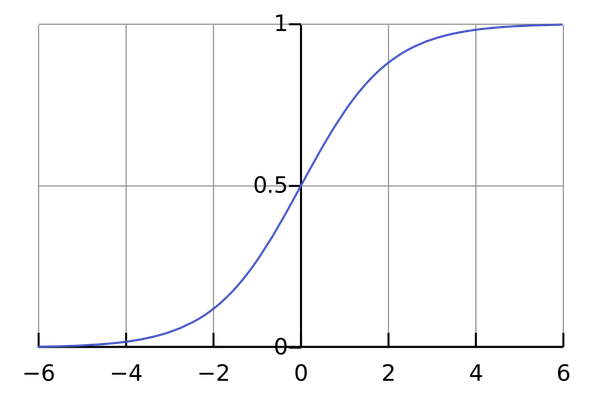
\includegraphics[width=0.5\textwidth]{./sigmoid.png}
\caption{The Sigmoid Function}
\end{figure}
\subsection{The Softmax Function}
We will now return to the predictive $p(y = c | x) \propto \exp(\theta_c^T x + c_c)$ to try to compute the normalizer $Z$: 
$$ p(y=c|x) = \frac{1}{Z} \exp(\theta_c^T x + b_c) $$
In general, we can compute the normal by summing over all our classes.
$$ Z(\theta) = \sum_{c'} = \exp(\theta_{c'}^T x + b_{c'}) $$
In practice, this summation is often computationally expensive. However, it is not necessary to compute this sum if we are only interested in the most likely class label given an input.

\smallskip

We call the resulting probability density function the \emph{softmax}: 
$$ \text{softmax}(z)_i = \frac{ \exp(z_i) }{ \sum_{i'} \exp(z_{i'})} $$
This function generalizes the sigmoid function to multiple classes/dimensions. 
\begin{figure}
\centering
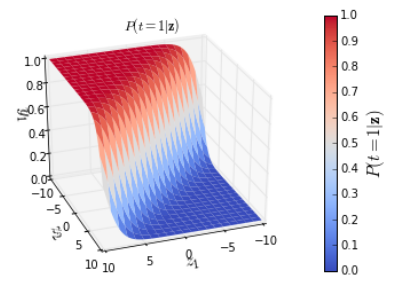
\includegraphics[width=0.5\textwidth]{./softmax.png}
\caption{The Softmax Function}
\end{figure}
We call it the "softmax" because we may think of it as a smooth, differentiable version of the function which simply returns $1$ for the most likely class (or argmax). 
\subsection{Discriminative Classification}
We may apply the mathematical tools developed in the generative classification setting discussed above to perform discriminative classification. In discriminative classification, we assume that our inputs $x$ are fixed, rather than coming from some probability distribution.

We take the maximum likelihood estimate, as in linear regression, given that $p(y = c | x) \propto \exp(\theta_c^T x)$: 
$$ \on{MLE}: \arg\!\max_{\theta} p(y | x, \theta) = \arg\!\max_{\theta} \sum_n \log \on{softmax} (\theta_c^T x_n) c_n $$
What are the advantages and disadvantages of this approach? The primary disadvantage compared to methods we have seen earlier is that this maximum likelihood estimate has \textit{no closed form}. It is also not clear how we might incorporate our prior (although there is recent work in this area). On the other hand, this equation is convex and it is easy (at least mathematically, not necessarily computationally) to compute gradients, so we may use gradient descent. 
\begin{align} 
    \frac{d (\cdot)}{d \theta_c} = \sum_n x_n \cdot \begin{cases} 1 - \text{softmax}(\theta_c ^T x) & \text{ if } y_n = c \\ \text{softmax}(\theta_c ^T x) & \text{otherwise} \end{cases} 
\end{align}
This model is known as \textbf{logistic regression} (even though it is used for classification, not regression) and is widely used in practice.

\medskip

\textbf{More Resources on Optimization}
\begin{itemize}
    \item Convex Optimization by Lieven Vandenberghe and Stephen P. Boyd
\end{itemize}

\end{document}



